\documentclass[10pt]{article}
\usepackage[utf8]{inputenc}
\usepackage{geometry}
\usepackage{varwidth}
\usepackage{graphicx, subcaption}
\usepackage{amsmath}
\usepackage{enumitem}
\usepackage{listings}
\usepackage[toc, page]{appendix}
\usepackage{booktabs, makecell, tabularx}
\usepackage{abstract}
\usepackage[dvipsnames,table,xcdraw]{xcolor}
\usepackage{tabularx}
\usepackage{lipsum}
\usepackage{natbib}
\usepackage{titling}
\usepackage{natbib}
\usepackage{ragged2e}
\usepackage{hyperref}
\usepackage{caption}

\bibliographystyle{abbrvnat}
\setcitestyle{authoryear,open={(},close={)}}
\renewcommand\theadfont{\small\bfseries}
\renewcommand\theadgape{}
\setcellgapes{3pt}
\newcolumntype{L}{>{\RaggedRight}X}
\newcolumntype{P}[1]{>{\raggedright\arraybackslash}p{#1}}
\captionsetup[table]{position=above, skip=0.5ex}
\graphicspath{ {./pictures/} }
\geometry{
a4paper,
total={170mm,237mm},
left=20mm,
top=20mm,
}

\newcounter{nalg}
\setcounter{nalg}{1}
\setcounter{page}{1}

\DeclareCaptionLabelFormat{algocaption}{\texbtf{Algorithm} \nalg}
\lstnewenvironment{algorithm}[1][] %defines the algorithm listing environment
{
\captionsetup{labelformat=algocaption,labelsep=colon}
\stepcounter{nalg}
\lstset{
mathescape=true,
frame=tB,
numbers=left,
numberstyle=\tiny,
basicstyle=\scriptsize,
xleftmargin=.04\textwidth,
keywordstyle=\color{black}\bfseries\em,
keywords={input, output, return, datatype, function, in, is, and, or, not, if, else, get, foreach, while, begin, end, end if}
#1
}
}{}


\title{Modeling civil violence : Influence of social networks \large \\ Agent-based Modelling \\University of Amsterdam\\}

\author{Daniël Vink (10675140), Floris de Vries (11710799), Roman Peerboom (10791523),\\ Sam Kuilboer (12442690), Viviane Desgrange (13337688)}

\date{}

\begin{document}


    \maketitle

    \begin{abstract}
    {\normalsize  This paper introduces an agent-based model of civil violence where a central authority tries to control violence among a population of civilian agents connected by a social network. It fixates on the influence of different network graph topologies, such as Erdos-Renyi, Watts-Strogatz \& Barbasi-Albert network, on civil violence. Additionally a special focus was on the Barabasi-Albert network, which contains so-called hubs, which are treated as the equivalent of a social media influencers. The impact of removing these influencers at the beginning of an outbreak is investigated.
    The impact of the addition of a social network on the model resulted in longer peak duration ($p<0.001$) and larger outbreak size ($p<0.001$). Between the model with different social networks implemented the differences were less clear. However, the Watts-Strogatz model had a HIGHER/LOWER peak duration ($p<0.01$) and the Erdos-Renyi had a larger outbreak size ($p<0.01$) compared to the other to models. The removal of influencers at the start of the outbreak in the model with a Barabasi-Albert social network resulted in a shorter outbreak duration ($p = 0.03$) and a smaller outbreak size ($p < 0.001$).
    }

        \smallskip
        \noindent
        {\normalsize \textbf{Keywords}: Agent-Based Modelling, Civil Violence, Social Network, Erdos-Renyi, Watts-Strogatz, Barabasi-Albert}
    \end{abstract}

    \newpage

    \section*{Introduction}
    Throughout the past decade, several governments were faced with a new type of civil violence, characterised by fast propagation and coordination on a wide scale. Examples of this are the Arab Spring back in 2011, the Yellow Vest movement in 2019, and the worldwide Black Lives Matter movement past year. The common characteristic of these uprisings is the important role that social media played in mobilizing the protesters. In this research, this phenomenon will be replicated in an agent-based model.
    This will be done by extending the original civil violence model of \cite{epstein2002}, in which citizens rebel against a central authority. In this simple model, Epstein did not consider any kind of social bond between agents. Nonetheless, the model gave interesting insights in crowd dynamics and how social violence is incited during protests.

    Over the last decade, social media has become increasingly important in everyday life. Following this growing importance of social media, more literature has appeared on the influence of the social network on population dynamics. The topic of influence of socials networks on civil violence in agent-based models is among them.

    One of the first publications on this topic is \cite{lemos2015}. This paper introduced simple networks, representing family and close friends, as well as \textit{influencer-agents} representing the media. The families were represented by a small undirected network (3-6 nodes) between agents. The media agents were represented by agents that moved close to fighting agents and `spread' this information through a wide directed graph of nodes. One of the important details to highlight is that the environment of the agents is composed of two lattices, one being a 2 dimensional grid created as in \cite{epstein2002} and one being a node-network which links agents to their family or media channel.

    To consider this new way of influence through this second network, \cite{lemos2015} replaced the number of active and quiet citizens localized in the agents vision area by an aggregation of the number of agents visible trough all present networks. He also extended the central authority legitimacy state variable through legitimacy feedback equation based on the above attributes. The paper considered multiple societal configurations, rural and urban, some having large families with limited media influence and vice versa.
    \cite{lemos2015} found that network influence did not changes the periodicity of the outburst however it increased their size; moreover the introduction of a legitimacy feedback changes the system behaviour with oscillations between equilibrium and permanent rebellion.

    In contrary to \cite{lemos2015} which covers the `traditional' media, \cite{fonoberova2019} used the second network as a way to incorporate undirected social networks, e.g., \textit{Facebook} or \textit{Twitter}. The underlying structure of the network is as described in \cite{watts1998}. This network, better known as the `small world network', tries to give an accurate representation of close relatives and some far-away friends. The network is build by connecting agents within a close neighborhood and rewire some of these connection with probability $\beta$. \cite{fonoberova2019} found this implementation led to more frequent large-scale violent outbursts, while for higher law-enforcement concentrations, outcomes depended most strongly on the number of local neighbours. One of the drawbacks of this approach is that the `Watts-Strogatz' network does not fully reflect a real-world network. As the distant-neighbours connections are randomly assigned, while in the real-world people tend to connect by \textit{following} central figures who typically already have many connections.

    Therefore, our research is aimed at the comparison of different network topologies that represent the real-world better, by observing the influence of these on the civil violence model. Additionally we study the role of well-connected individuals, the equivalent of influencers in the real world, in the Barabasi-Albert network on the emergence of outburst, as well as the consequences of manipulating these agent to control civil violence.

% In our paper, we considered a similar approach as \cite{lemos2015} given that the integration of the social network into the state variables is the same as we seek. However, in contrary to \cite{lemos2015} in which the 'traditional' media is incorporated, we want to incorporate the social media. Therefore, a recent publication of \cite{fonoberova2019} caught our attention. \cite{fonoberova2019} used the second network as a way to incorporate undirected social network, for example representing a social media network as \textit{Facebook} or \textit{Twitter}. The underlying structure of the network is as described in \cite{watts1998}. This network, better known as the 'small world network', tries to give an accurate representation of close relatives and some far-away friends. The network is build by connecting agents within a close neighborhood and rewire some of these connection with probability $\beta$. The results showed that this implementation lead to more frequent large-scale violent outbursts, while for higher law-enforcement concentrations, outcomes depended most strongly on the number of local neighbours. One of the drawbacks of this approach is that the 'Watts-Strogatz' network does not fully reflect a real-world network. As the distant-neighbours connections are randomly assigned, while in the real-world people tend to connect by \textit{following} central figures who typically already have many connections.

    \newpage

    \section*{Theoretical background}

    The first network we are implementing is the \cite{erdHos1960evolution} network. In contrary to the Watts-Strogatz network, this network is randomly created. For every node, all the possible edges are evaluated with a certain probability $P$. The final graph represents random connections between nodes and a relatively low cluster coefficient. The degree distribution of the nodes follows a normal distribution. Although these two factors are drawbacks when it comes to reflect the real-world. The random connections could reflect the large groups of activists most protesters are connected to.\\

    The second network we want to introduce is the Barabasi-Albert Network. This network resolves the two major draw backs of the other networks, being the absence of a power-law distribution and low clustering coefficients. \cite{barabasi2009scale} had the network created node by node. These new nodes would not randomly select connections, however they have a tendency to make interactions to a node which already has a lot of connections, a phenomenon called preferential attachment. The result is a network in which a small number of nodes is well connected, while the vast majority has a relatively small number of connections. This automatically leads to the question what the influence is of these well-connected agents.

    \begin{figure}[h]
        \makebox[\textwidth][c]{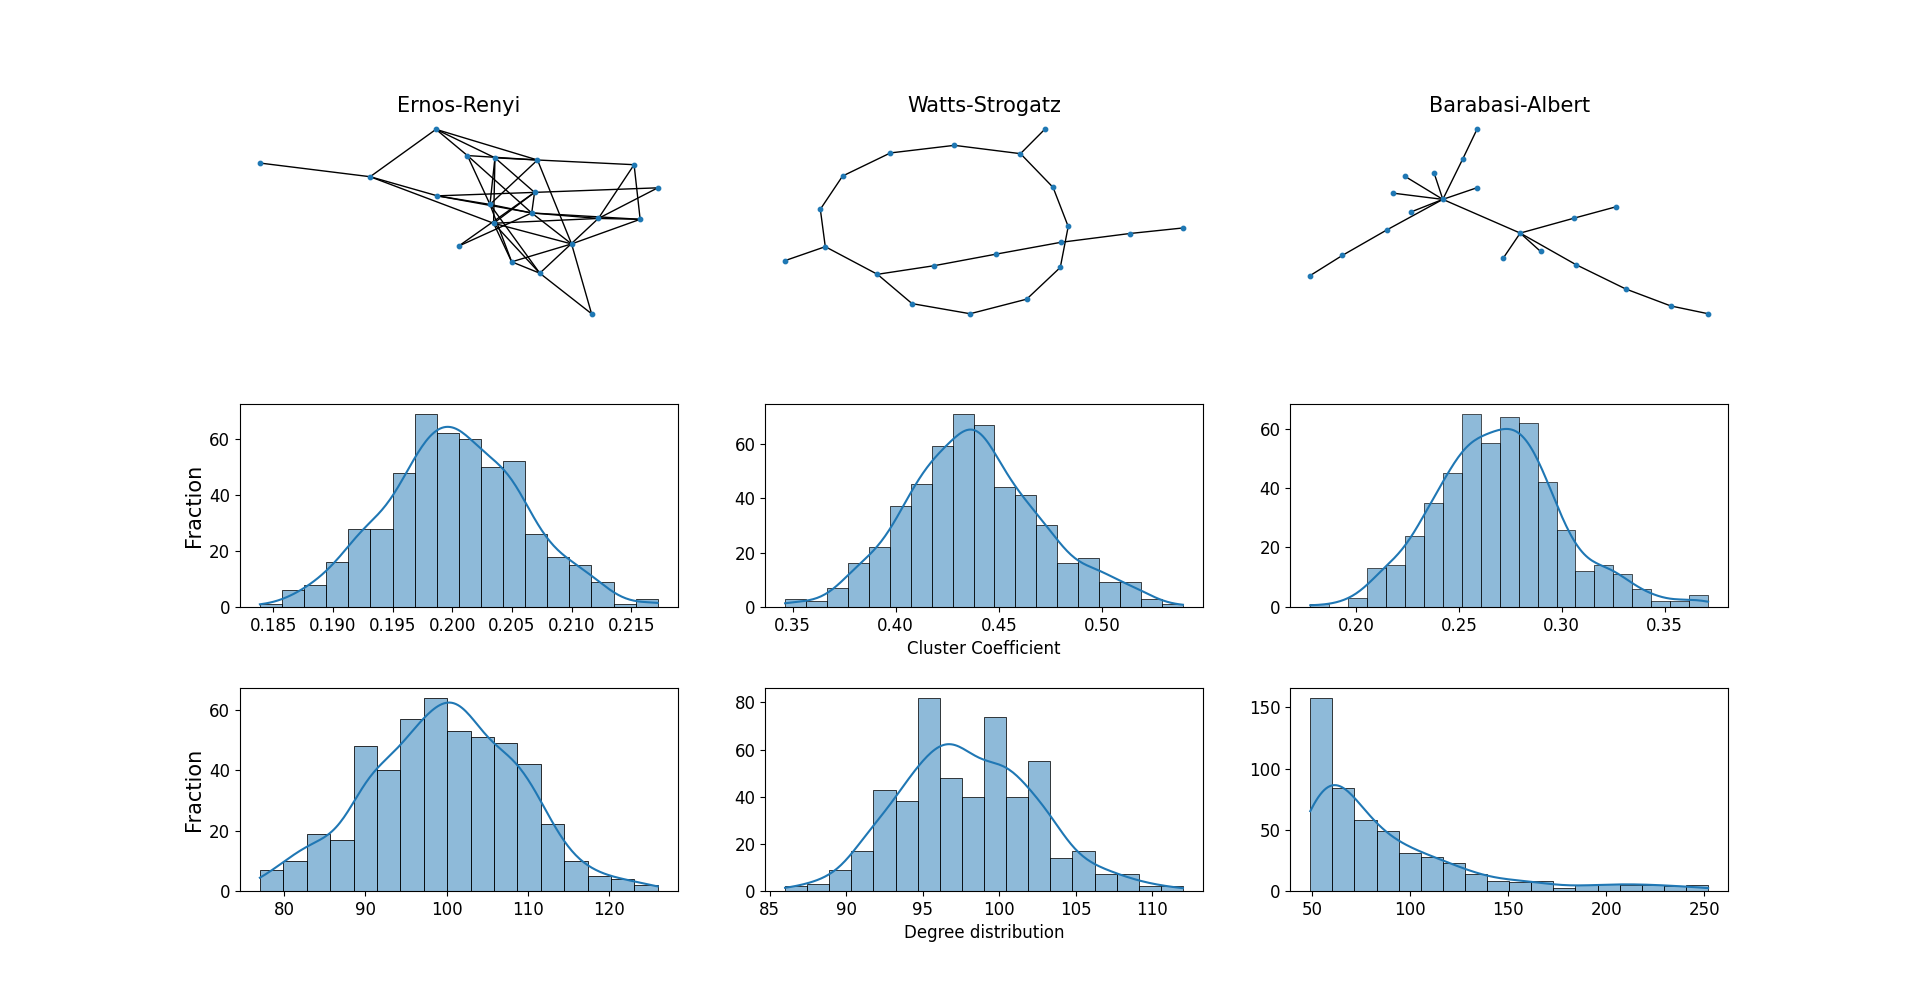
\includegraphics[width=1.3\textwidth]{pictures/network3.png}}%
        \caption{Representation of the Ernos-Renyi, Watts-Strogatz and Barabasi-Albert network. The figures in the first row are minimised representations of the networks used in the experiments. The Barabasi-Albert network is the only scale-free network due the power-law distributed connections per node. The cluster-coefficient of the Watts-Strogatz network is the highest due the fact that every node is at least connected to his closest neighbours. }
        \label{fig:key}
    \end{figure}

    \newpage

    \section{Overview}

    \subsection{Purpose}

    As an extension of the civil violence model from \citet{epstein2002}, study the influence of different network topologies on civil violence. As a follow-up, examine the suitability of the manipulation of influencer-agents that emerge in the Barabasi-Albert network, as a potential outbreak prevention technique.

    \subsection{Entities, state variables, and scales}

    The civil violence model contains two types of agents: the civilian and the law
    enforcement officer (the cop). These two agents are defined by state variables and regulated by rules, interacting between them or with the model (See Table \ref{table:parameter_descriptions} for details).

    \subsubsection{Civilian Agents}
    \label{section:civilian_entity}

    \begin{figure}[h]
        \centering
        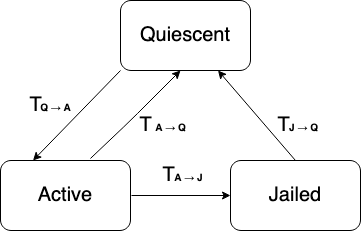
\includegraphics[width=.4\textwidth]{pictures/entities_state_variables_scales/citizen_agents/citizen_agent_2.png}
        \captionsetup{width=.4\textwidth}
        \caption{State-transition rules of civilian agent. The transition $T_{Q \rightarrow A}$ and $T_{A \rightarrow Q}$ depends on the application of the citizen Rule A.}
        \label{fig:state_transition_rule_civilian}
    \end{figure}

    Civilian agents in the civil violence model can be in one of three different possible states, the same as in the original model of \citet{epstein2002}: \emph{quiescent}, \emph{active}, or \emph{jailed}. A quiescent agent is not in revolt and just moves around the grid randomly. At every step, it makes the decision whether or not to be active. It does so by weighing its individual \emph{grievance} (G) against its fear of being arrested, the \emph{net risk perception} (N). The grievance of an individual is a combination of individual \emph{hardship} (H) and \emph{global legitimacy} (L) of the government:

    \begin{equation}
        G = H(1 - L)
    \end{equation}

    This formula does not differ from the one in the model in \cite{epstein2002}. However, we calculate the hardship and the legitimacy in different ways, which we will introduce in two coming paragraphs. The \emph{net risk perception} ($N$) is calculated by multiplying the \emph{estimated arrest probability} ($P$) of the agent in the case that it turns active with the agent's \emph{individual risk aversion} ($R$), such that:
    \begin{equation}
        N = RP
    \end{equation}
    The \emph{risk aversion} R is drawn from U(0,1). The \emph{estimated arrest probability} is $P = 1 - exp( - k \lfloor\frac{C_v}{A_v + 1}\rceil)$, where $C_v$ and $A_v$ represents the \emph{number of cops and citizens} in the \emph{agent's vision} $v_a$, and the constant $k = 2.3$ insure the plausibility of $P$. We highlight the fact that the equation is slightly updated from \citet{epstein2002}. The cop-to-agent ratio also includes the agent himself as he estimates the probability of being arrested. This resolves the risk of dividing by zero and ensure when $C_v = A_v$ then $P = 0.9$. This leads us to the main citizen state transition rule:

    \begin{quote}
        \textbf{Rule A}: If  $G - N > T$, the agent is active ($T_{Q \rightarrow A}$); otherwise is quiescent ($T_{A \rightarrow Q}$).
    \end{quote}

    If the result of this exceeds the \emph{agent's individual threshold}, $T = 0.1$ in our case, the quiescent agent becomes active. These calculations are also performed for every active agent at every step and if its level of grievance lowers to the point that the threshold is not reached, the agent turns quiescent. The dynamics that were just described are identical to the model in \cite{epstein2002}.

    \paragraph{Hardship}
    As a reminder, the Epstein's model \emph{Grievance} of a specific agent is $G = H(1 - L)$, in which the values for \emph{Hardship} (H) and \emph{Legitimacy} (L) are both randomly drawn from the uniform distribution $U(0,1)$. In our model, we extended this by introducing time-dependent values for $H(i,t)$ and $L(t)$. $H(i,t)$ is composed of $H_{endo}$, drawn from the uniform distribution $U(0, 1)$, which stands for the individual endogenous hardship and the contagious hardship $H_{contg}(i,t)$ defined by the equation:

    \begin{align}
        H(i, t) &= H_{endo}(i) + H_{contg}(i, t)\\
        H_{contg}(i,t) &= H_{contg}(i,t - \delta t) + \sum\limits_{j = 1}^{N_{ir, A}} h_{ij}
    \end{align}

    Where $\sum\limits_{j = 1}^{N_{ir, A}} h_{ij}$ represents the received hardship of an agent from the active agents that it is connected to. $h_{ij}$, the hardship influence of agent j on agent i is given by the equation:

    \begin{equation}
        h_{ij} = \Delta t  * A_i * B_j * E_j*\beta
        \label{eq:extended_hardship}
    \end{equation}

    \begin{itemize}[noitemsep]
        \item $A_i$ is a parameter of agent i that indicates its receptiveness to influence of other agents.
        \item $B_j$ is a parameter of agent j that indicates its capability to influence other agents.
        \item $E_j$ represents the intensity at which agent j expresses its hardship.
        \item $\beta$ corresponds to the transmission rate, an intrinsic value of the contagiousness of violence. As this research does not compare different ways of spreading violence, the effects of different values for $\beta$ are beyond the scope of this research and we set this parameter fixed at 0.5.
    \end{itemize}


    $A_i$, $B_j$ \& $E_j$ are drawn from uniform distribution $U(0,1)$. This model for grievance is an adjusted version of a model on collective violence outbursts by \citet{huang2018}. The underlying idea is derived from biological processes representing the spread of an infectious disease \citet{fu2014simulation}.

    \paragraph{Legitimacy}
    In the standard Epstein model, the \emph{perceived legitimacy} $L_0$ of the government is fixed for every time step. In real situations however, it makes sense that the perception of a government's legitimacy is perceived differently over time based on the actions of that government. We integrated this idea into our model by making the legitimacy of the government dependent on the amount of people that were jailed in the last couple of time steps. The legitimacy $L_B(t)$ is calculated by:

    \begin{equation}
        L_B(t) = L_0(1- \sum\limits_{i = 1}^{m} \beta^i_i)
    \end{equation}
    \begin{equation}
        \beta_i = \frac{Amount\ of\ agents\ put\ in\ jail\ in\ period\ i}{Amount\ of\ agents\ not\ in\ jail\ at\ the\ start\ of\ period\ i}
    \end{equation}

    These formulas are adjusted versions of ideas in the working paper of \cite{epstein2001modeling}. They ensure that the perceived legitimacy of the government is a direct result of the actions of the government.


    \subsubsection{Influencers}
    \label{section:influencer_entity}

    The influencer agents are a subset of citizen agents. However, the principal attribute which segregate influencers from civilians is the number of connection to other agents in the social network. The idea behind making the influencer an extension of the civilian agent instead of a separated entity like a media or a propaganda agent, can be track down to the fact that the influencers do not follow similar 'professional' rules to media/propaganda entities. Media/propaganda entities from \citet{lemos2015} look for activity clusters in the environment, and spread the 'information' to civilian agents through a directed graph. However, the influencer citizen can be influenced by other connected agents and can change between the active quiescent or jailed state.

    Therefore, as a way to control our experiments in different context the civilian agent was extended with the following rules and attributes:
    \begin{itemize}
        \item Civilian agents are marked as \emph{influencer} beyond a threshold $T_c$, fixed at initialisation of the model (See Section \ref{section:model_initialisation}).
        \item At initialisation of the social network, influencer agents are listed.
        % \item A \emph{jailable} attribute let us specify if an influencer agent is jailable or not by cop agent.
        \item Add and remove methods are implemented to jail influencer agents at the start of an outbreak.
    \end{itemize}


    \subsubsection{Cops}
    \label{section:cop_entity}

    Cops also move around the grid. Every time step, cops check for active agents in their vision $v_c$; if an active agent is present, the cop arrests this agent and moves to that spot. Otherwise, it continues its search for active agents by moving to another random accessible point on the grid.

    \begin{quote}
        \textbf{Rule C}: Inspect cells in the cop vision $v_c$. If any active citizens present, move there and arrest him. Otherwise move to a random spot.\\
        \textbf{Rule J}: Arrested active agents are jailed ($T_{A \rightarrow J}$) for the duration of its sentence.
    \end{quote}

    During imprisonment the civilian agent does not perform any steps and is removed from the grid for the duration of its sentence. The duration of the jail sentence is randomly drawn from a uniform distribution between 0 and the maximal jail sentence $J_{max}$.

    \begin{table}[h]
        \centering
        \begin{tabular}{||>{\bfseries}l c c || >{\bfseries}l c c||}
            \hline
            Parameter & Symbol & Bounds & Parameter & Symbol & Bounds \\
            \hline
            \hline
            Hardship & H & $[0,1]$ & Transmission rate & $\beta$ & $[0,1]$ \\
            Legitimacy & L & $[0,1]$ & Activity threshold & $T_c$ & $[0,1]$ \\
            Grievance & G & $[0,1]$ & Estimated arrest probability & P & $[0,1]$ \\
            Risk aversion & R & $[0,1]$ & Cop to agent ratio & $\frac{C_v}{A_v + 1}$ & $[0,\infty[$ \\
            Net risk perception & N & $[0,1]$ & Agent vision & $v_a$ & $[1, \infty[$ \\
            Susceptibility & $A_i$ & $[0, 1]$ & Cop vision & $v_c$ & $[1, \infty[$ \\
            Influence & $B_j$ & $[0,1]$ & Agent density & $d_a$ & $[0,1]$ \\
            Expression intensity & $E_j$ & $[0,1]$ & Cop density & $d_c$ & $[0,1]$ \\
            Maximal jail term & $J_{max}$ & $[0, \infty]$ & Jail term & J & $[0,J_{max}]$ \\
            Arrest probability constant & k & 2.3 & Lifetime & max\_iters & $[1, \infty[$ \\
            \hline
        \end{tabular}
        \caption{Civil violence model parameters, symbols and theoretical bounds}
        \label{table:parameter_descriptions}
    \end{table}

    \subsection{Process overview and scheduling}

    Our civil violence model is a discrete time model with a fixed limit defined at initialisation of the simulation. At each iteration, the model calls agents (civilian \& cops) in a random order to let them run their action. After iterating over all running agents, the model will update the central authority \emph{legitimacy} state variable $L$. In the next section, the model counts the number of active agents and determines if the outbreak threshold is exceeded. The model keeps track of the number of outbreaks for each simulation. The model is able to imprison the influencer agents at the start of those outbreaks. This will be done in the experiments that focus on the effect of removing influencer agents at the start of an outbreak. Finally, if the iteration step reached the maximal iteration parameter, the simulation stops. See details from flow chart in Appendix \ref{appendix:A} Figure \ref{fig:flow_chart_model}.

    In every step a civilian agent will first update its current \emph{hardship} attribute (See Section \ref{section:civilian_entity}) before keeping track of its neighbors within its vision (cardinal directions) and the social network. From these information the civilian agent update its status according to the \emph{rule A} (See Section \ref{section:civilian_entity}). Eventually it will move randomly in one of the accessible empty cells around him (\emph{rule M}).Interaction between civilian agents will only leads to update of their state variables (\emph{Grievance}, \emph{Hardship}, etc.), while interaction with cops might results in imprisonment.


    \begin{algorithm}[caption = {Role: Civilian agent}]
        Require: Civilian Agent A, MultiGrid G
        if A.jail_sentence:
        A.jail_sentence -= 1

        if A.jail_sentence == 0:
        A.state = QUIESCENT
        A.hardship_cont = 0
        Place A in G
        return
        end if
        end if

        update A.hardship
        A.neighbors     = Agents in Agent vision
        A.empty_cells   = Empty cells in Agent vision
        update A.grievance

        rule_a = A.grievance - A.net_risk > A.threshold
        if A.state is QUIESCENT and rule_a:
        A.state = ACTIVE
        else if A.state is ACTIVE and not rule_a:
        A.state = QUIESCENT

        get random cell C in A.empty_cells
        move A to C
    \end{algorithm}

    \begin{algorithm}[caption = {Role: Cop agent}]
        Require: Cop Agent P, MultiGrid G
        P.neighbors   = Agents in Cop vision
        P.empty_cells = Empty cells in Cop vision
        active_neighbors = []

        for A in P.neighbors:
        if A is CITIZEN and A.state is ACTIVE and A.jail_sentence is 0 and A.jailable:
        add A in active_neighbors

        if active_neighbors:
        A = get random agent in active_neighbors
        A.state = JAILED
        A.jail_sentence = random(1, max_jail_term)
        remove A from G
        move P to A
        return
        else
        get random cell C in P.empty_cells
        move P to C
    \end{algorithm}

    \section{Design concept}
    \subsection{Basic principles}
    Civil uprisings are the results of dynamic, social processes. People encourage each other to take to the streets in a collective manner. This phenomenon has been captured in agent-based models by previous researchers, such as the model that formed the basis of our model by \cite{epstein2001modeling}. Recent uprisings have shown a new dynamic: the use of social media. People that normally would have had no form of contact can influence each other through these online channels. An example of this is the Arab Spring, where social media played a large role in mobilizing people to join the protests \cite{howard2011opening}. Our model extends the `old' model where agents only influence other agents in their proximity with this new dynamic of influence regardless of the place on the grid.

    To replicate these social media connections, the three different types of networks that were discussed in the theoretical background correspond to the network structure that will provide the additional connection between the civilian agents.

    \subsection{Emergence}
    The output of our model is the size and dynamics of civil uprisings. Hence, the amount of active agents through time will be observed. The threshold for an outburst is at least fifty active agents on the grid. Concretely, the output consists of the outbreak frequency, outbreak peak heights and outbreak duration.

    \subsection{Adaptation}
    There is no difference between the places on the grid so the agents on it have no specific adaptation for it. All agents on the grid have approximately the same amount of agents in their proximity since the grid has the torus property.

    \subsection{Objectives}
    Agents have no specific objectives to complete. They purely react on situations and therefore, they also cannot learn and predict.

    \subsection{Sensing}
    Every time step, a civilian agent calculates its own hardship by observing the hardship of other agents connected to him on the social network. It also observes the global legitimacy of the government and uses these two values to determine its personal grievance. To calculate its arrest probability it also observes the amount of active agents and cops in its neighborhood.

    A cop agent actively checks its surrounding cells on the grid within its vision for active agents to arrest. If there are no active civilians within its vision, the cop moves to an empty cell instead.

    \subsection{Interaction}
    The model includes two possible types of interactions between agents: between two civilian agents and between a civilian and a cop. At every time step, citizens exercise influence on each other leading to an increase in contagious hardship. When an active agent and a cop enter each other's neighborhood, an interaction in the form of an arrest of the active agent takes place.

    \subsection{Stochasticity}
    Agents and cops randomly move around the grid, therefore the frequency of encounters between cops and citizens that lead to arrests is stochastic. Additionally, when multiple active agents are present, the cop randomly chooses one to arrest. The jail term is also random. The global legitimacy and personal grievance are dependent on these stochastic encounters.

    There are a number of parameters for agents relating to contagious hardship that are randomly drawn from a uniform distribution, these include: Initial personal hardship, receptiveness to influence of agents, capability to influence other agents and intensity at which hardship is expressed.

    Connecting the agents is also a stochastic process, no matter the type of network.

    \subsection{Collectives}
    When agents are active at the same time they are seen as part of the same uprising. It does not matter whether or not they are connected or close to each other on the grid, in both cases they influence each other's hardship.

    \subsection{Observation}
    For every civilian agent these variables are stored: Status of being active or not, level of hardship, grievance, its place on the grid and number of connections. Only their place on the grid will be stored for cop agents. For the whole model, the global legitimacy, the average number of connections and the number of influencers are stored.

    \section{Details}

    \subsection{Initialization}
    \label{section:model_initialisation}

    For our experiments, the civil violence model is initialized with the attributes from the Table \ref{table:parameter_initialization}.\\
    As previously discussed, the civilian's endogenous hardship and risk aversion, as well as the influence, susceptibility and expression intensity with respect to the social network are drawn from a uniform distribution $U(0, 1)$.

    \begin{table}[h]
        \centering
        \begin{tabular}{||>{\bfseries}l c ||}
            \hline
            Parameter & Initial value \\
            \hline
            \hline
            Grid & 40 $\times$ 40 \\
            Torus & True \\
            Lifetime & 200 steps \\
            Initial legitimacy & 0.8 \\
            Arrest probability k & 2.3 \\
            Civilian density & 0.7 \\
            Initial active civilian density & 0.01 \\
            Cop density & 0.04 \\
            Civilian vision & 7 \\
            Cop vision & 7 \\
            Active threshold & 0.1 \\
            Influencer threshold & 150 \\
            Maximum jail term & 30 \\
            Activation schedule & random \\
            Network directed & False \\
            Edge creation probability p & 0.1 \\
            Rewiring probability $p_w$ & 0.1 \\
            Outbreak threshold & 50 \\
            \hline
        \end{tabular}
        \caption{Civil violence model initial values }
        \label{table:parameter_initialization}
    \end{table}

    \subsection{Input data}
    The model uses no additional input data.

    \subsection{Submodels}
    There is no submodels defined in this implementation.

    \newpage

    \section{Results}

    \subsection{Sensitivity analysis}
    To investigate how the parameters influence our model a local (Figure \ref{fig:SA}) and global sensitivity analysis (Figure \ref{fig:global_sa}) was performed. The analysis were done on the model without a social network implemented, to minimise bias for parameter initialisation for one of the models. As output parameter the amount of outbreaks was used. It was reasoned that a sufficient amount of outbreaks needs to take place, to conclude that the models works.

    \subsubsection{One factor at a time sensitivity analysis}
    In the one factor at a time (OFAT) analysis five parameters were investigated: the active threshold, initial legitimacy, max jail term, citizen vision \& cop vision \ref{fig:SA}. For the active threshold a value around 0.1 should be chosen, otherwise the threshold for agents to become is too high and no outbreaks will occur. For the initial authority legitimacy the value should be lower than 0.9 for outbreaks to occur, otherwise the legitimacy is too high and no citizen will become active. The max jail term should be above 20, otherwise there will be one continuous outbreak. However, it should not become too large, then less outbreaks will occur since it takes too long before enough people have returned to the grid. For citizen vision a vision of 5-7 resulted in the highest number of outbreaks. A citizen should be able to see at least several other citizens, however, when it can see too much the amount of cops in its vision get too high and people, if they get active at all, will only become active for a short period of time, before they become quiescent again. For the cop vision the value should not be below three, since then cops won't be able to arrest the active citizens effectively and a continuous outbreak will be present. If the value on the other hand gets too large, the cops will jail the present active citizens immediately before an outbreak can occur. For the cop vision a value around 5-7 resulted in the highest number of outbreaks.

    Next our findings for the optimal values were compared with earlier research that investigated the civil violence model or extensions of it by \cite{epstein2002}, \cite{fonoberova2019}, \cite{huang2018} \& \cite{lemos2015}. All of them used an active threshold of 0.1. For initial legitimacy values around 0.8 were used. The max jail term however differed between the studies, but our optimum at 30 was in line with the value used by \cite{lemos2015}. For the citizen and cop vision also different values are used in the earlier studies. Our optimal value of 5-7 for agent \& cop vision is in the range of parameter values used, and is the same as used by \cite{lemos2015} \& \cite{epstein2002}.

    \begin{figure}[h]
        \centering
        \begin{subfigure}[b]{.4\linewidth}
            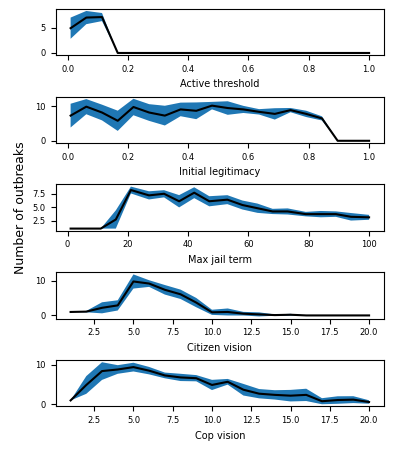
\includegraphics[width=\textwidth]{pictures/Sensitivity_analysis/Local SA2.png}
        \end{subfigure}
        \captionsetup{width=.5\linewidth}
        \caption{One factor at a time sensitivity analysis performed on the model without a social network implemented. As an output variable the number of outbreaks was used.}
        \label{fig:SA}
    \end{figure}

    \subsubsection{Sobol sensitivity analysis}
    To investigate the interactions of the different parameters in the model a global sensitivity analysis was performed on three different parameters: the max jail term, initial legitimacy \& active threshold. Only the first order sensitivity index of the active threshold was significantly different from zero, max jail term and initial legitimacy did not differ significantly (Figure \ref{fig:global_sa}). However, when we look into the total order sensitivity index all three parameters had a significant impact on the model. This indicates that the specified value for these parameters does matter, largely due to interactions with other parameter values.

    \begin{figure}[h!]
        \centering
        \begin{subfigure}[b]{.45\linewidth}
            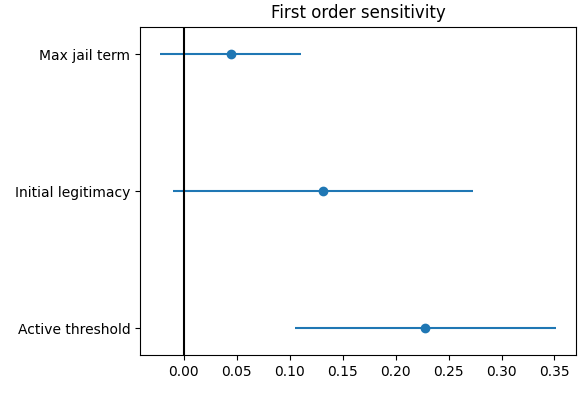
\includegraphics[width=\textwidth]{pictures/Sensitivity_analysis/Global SA_first2.png}
            % \caption{Global First Order SA}
            \label{fig:global_sa_first order}
        \end{subfigure}
        \begin{subfigure}[b]{.45\linewidth}
            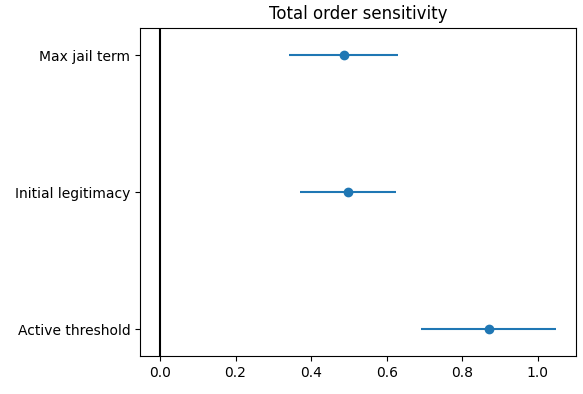
\includegraphics[width=\textwidth]{pictures/Sensitivity_analysis/Global SA_total2.png}
            % \caption{Global Total Order SA}
            \label{fig:to_SA}
        \end{subfigure}
        \captionsetup{width=0.9\linewidth}
        \caption{Sobol sensitivity analysis performed on the model without a social network implemented. The left graph displays the first order sensitivity index and the right graph the total order sensitivity index. As an output variable the number of outbreaks was used.}
        \label{fig:global_sa}
    \end{figure}

    \subsection{Comparing Network Structures}
    The results obtained form the model with different social networks implemented are displayed in Figure \ref{fig:duration} and \ref{fig:size}. The three models with a network implemented had comparable behaviour. The most profound difference was between the in- and exclusion of a social network structure. The reference model without a network had a significant shorter peak duration (for all $ p < 0.001$) and a significant lower peak height (for all $ p < 0.001$) compared to the models with a social network implemented.

    Furthermore, the implementation of the Watts-Strogatz network resulted in a significantly HIGHER/LOWER compared to the implementation of the other two networks (for both $p<0.01$). No difference was found between the model with the Barabasi-Albert and the Erdos-Renyi network ($p = 0.3$) in peak duration. However, the outbreak size in the model with the Erdos-Renyi network implemented was significantly higher compared to the size in the other two models (for both $p<0.01$). The implementation of the Barabasi-Albert or the Watts-Strogatz model did not result in different outbreak sizes ($p = 0.4$).

% While the behavior between the different models is similar, it is worth noting that the Erdoys-Reyni model had the highest average outbreak size. The Barabasi-Albert model seemed to be slightly more densely distributed around its average outbreak duration than the other network models.

    \begin{figure}[h!]
        \centering
        \begin{subfigure}[b]{.45\linewidth}
            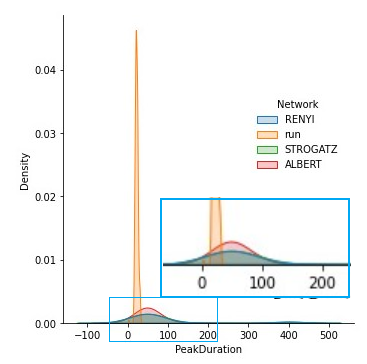
\includegraphics[width=\textwidth]{pictures/Results/duration_comparison.png}
            \caption{The outbreak duration per model with the different social networks implemented. The models with a social network had a significantly higher peak duration compared to the model without a social network (for all $p < 0.001$). Furthermore the Watts-Strogatz model had a significantly HIGHER/LOWER (NOT VISIBLE IN THIS GRAPH) peak duration compared to the Barabasi-Albert \& Erdos-Renyi model (for both $p < 0.01$). No significant difference was found between the Barabasi-Albert \& Erdos-Renyi model ($p = 0.3$). }
            \label{fig:duration}
        \end{subfigure}
        \begin{subfigure}[b]{.45\linewidth}
            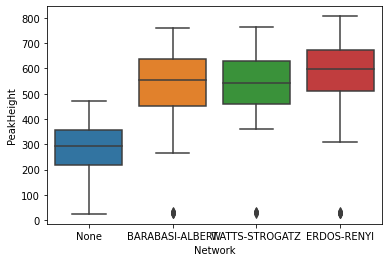
\includegraphics[width=\textwidth]{pictures/Results/BP_peak_height.png}
            \caption{The outbreak size per model with the different social networks implemented. The models with a social network implemented had a significantly higher peak duration compared to the model without a social network (for all $p < 0.001$). Furthermore, the Erdos-Renyi network resulted in a significantly higher peak height compared to the Barabasi-Albert \& Watts-Strogatz model (for both $p < 0.01$). No significant difference was found between the Barabasi-Albert \& Watts-Strogatz model ($p = 0.4$). }
            \label{fig:size}
        \end{subfigure}
        \captionsetup{width=0.9\linewidth}
        \caption{The outbreak duration and outbreak size for the model with different social networks implemented.}
        \label{fig:results}
    \end{figure}

    \subsection{Removing Influencers}
    The natural structure of the Barabasi-Albert network contains certain hubs: nodes with a significant higher amount of connections than the average node. The experiment pertaining the removal of \textit{influencers} from the Barabasi-Albert network was set up in a way to investigate if the targeted removal of influential agent could prevent mass outbreaks from occurring. This prompt removal is ensured by jailing all influencer-agents in the model for a randomly sampled period of time just before the model reaches the outbreak threshold. The outbreak threshold was set at fifty and the threshold for influencer agents to be removed at thirty. The removal of the influencers did not result in less outbreak, however, the outbreaks that did occur were shorter  ($p = 0.03$) and smaller ($p < 0.001$). %Remarkably, the model where influencers were removed has two outliers with extreme long outbreak duration that both exceed the maximum recorded duration of the reference model.

    \begin{figure}[b!]
        \centering
        \begin{subfigure}[b]{.45\linewidth}
            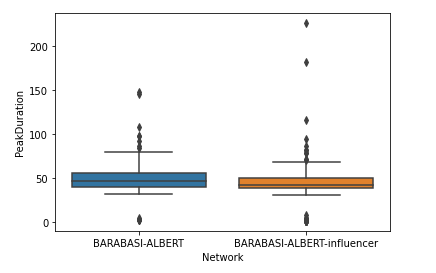
\includegraphics[width=\textwidth]{pictures/Results/influencer_removal_duration.jpg}
            \caption{The outbreak duration for the Barabasi-Albert model with and without removal of the influencers at the start of the outbreak. The model where the influencers were removed had a significantly shorter peak duration ($p= 0.03$).}
            \label{fig:ba_boxb}
        \end{subfigure}
        \begin{subfigure}[b]{.45\linewidth}
            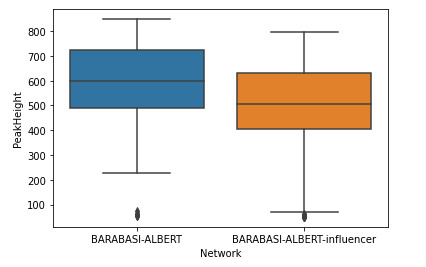
\includegraphics[width=\textwidth]{pictures/Results/influencer_removal.jpg}
            \caption{The outbreak size for the Barabasi-Albert model with and without removal of the influencers at the start of the outbreak. The model where the influencers were removed had a significantly lower peak height ($p < 0.001$).}
            \label{fig:ba_boxa}
        \end{subfigure}
        \captionsetup{width = 0.9\linewidth}
        \caption{The outbreak duration and outbreak size for the model with the Barabasi-Albert model was implemented. In the boxplots colored in blue the influencers were not removed at the start of an outbreak, whereas in the orange boxplot they were.}
        \label{fig:inf_comp}
    \end{figure}

    Closer inspection of peak heights of the two models (Figure \ref{fig:inf_dens}) display that the influencer removal model has generated an additional densely distributed area around the outbreak threshold. This bimodal distribution can explain the outliers around the lower outbreak sizes that are present in Figure \ref{fig:ba_boxa}. While in the influencer removal model relatively more smaller outbreaks are present, the bulk of the outbreaks retain their relatively large peak heights. Probably this can be attributed to the fact that the perceived legitimacy of the system decreases, when the amount of jailed citizens increases.

    \begin{figure}
        \centering
        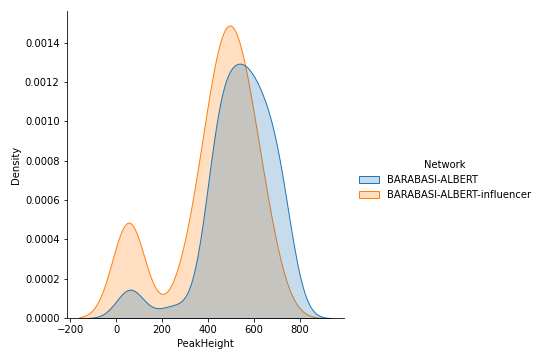
\includegraphics[width=.50\textwidth]{pictures/Results/only2density.png}
        \captionsetup{width=0.5\linewidth}
        \caption{Bimodal distribution of outbreak peak height for the Barabasi-Albert model with and without removal of the influencer agents at the start of the outbreak. Emerging civil violence (mode at 50), it appears that removing influencer agents prevent outbreaks to spread. Outbreaks which spreads to a majority of the population (mode at 500), the removal of influencer agents do not generate significant difference.}
        \label{fig:inf_dens}
    \end{figure}

    \newpage

    \section{Conclusion}

    This paper started with the assumption that expansion of civil violence model introduce by Epstein with social networks would leads to broad difference depending on the graph topology used to represent this network. It also started with the presumption that well-connected agents were one of the main points of interest to control spreading of civil violence by a central authority.\\
    In the midst of our experiments, we discovered that although the model output does not differ significantly between the tested network structures, the addition of a social network does in fact lead to a bimodal distribution with lower frequency of longer and larger outbreaks. Thus, the inclusion of a social network leads to a definite change in social dynamics in the model.\\
    Subsequent discoveries involve the impact of well-connected, aka. Influencer, agents on the diffusion of outbreaks. While a large number of outbreaks are effectively snuffed out at their inception with the removal of influencers; violent outbreaks that are well underway remain relatively unaffected. This fact could be attributed to the fact that the perceived legitimacy of the system decreases, when the number of jailed citizens increases. These latest findings point the idea that targeted jailing at an early stage might not be an effective tactic to prevent large outbreaks, however it also raises some interrogations on the method used for the spread of information in social network, given that average agent and well-connected influence strength over hardship contagion does not differ much.

% The finding that most large outbreaks stay present in the influencer removal model can probably  be attributed to the fact that the perceived legitimacy of the system decreases, when the amount of jailed citizens increases.

% Although the model output does not differ significantly between the tested network structures, the addition of a social network does in fact lead to a lower frequency of longer and larger outbreaks. Thus, the inclusion of a social network leads to a definite change in social dynamics in the model.

% From this emphasized dynamic can be concluded that a large amount of outbreaks are effectively snuffed out at their inception. While violent outbreaks that are well underway remain relatively unaffected by the removal of influencers, their targeted jailing at an early stage appears to be an effective tactic to prevent outbreaks from happening at all.




    \subsection{Future Work}
    A possibility to improve further on the concept of influencers is to check for their parameter $\beta_i$, the parameter that controls the capability of the agent to influence other agents in the contagious hardship formula. Right now, the only requirement to be deemed as an influencer is to have a lot of connections. However, the impact of the value of $\beta_i$ on the total influence of an agent is big as well, that is the influence strength between average civilian agents and influencer agents  on hardship contagion does not differ. An improvement on the model could be to take this parameter into account. Furthermore, it could be interesting to change the value for the $\beta_i$ of influencer agents over different runs, to see how important it is that influencer agents are able to convince their followers.\\

    An additional idea for future research is to introduce a parameter that controls the behaviour of cops. For example, a parameter that gives a possibility for a cop to arrest an active agent in its neighborhood, instead of cops always arresting when they can. This way, the impact of the strictness of a government could be investigated. The dynamic between the legitimacy feedback and arrests of active agents could lead to interesting results.

    \subsection{Source code}

    For further details, the source code of this agent-based model is publicly available on GitHub at the address: \url{https://github.com/vdesgrange/agent_based_modelling}

    \bibliography{ref}

    \newpage

    \appendix
    \section{Process overview and scheduling}
    \vspace*{0pt}
    \label{appendix:A}

    \begin{figure}[ht!]
        \centering
        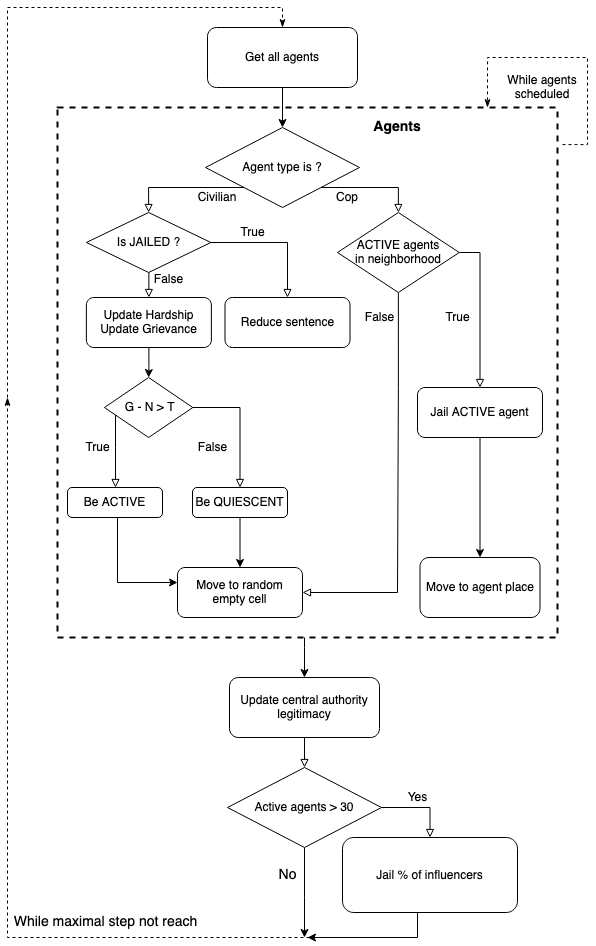
\includegraphics[width=.75\linewidth]{pictures/process_overview_scheduling/civil_violence_flow_chart_2.png}
        \caption{Flow chart of the civil violence model. Civilian and cops only common action is the verification of surround neighbors, they later differ in the update of their own state variable as well as their movements.}
        \label{fig:flow_chart_model}
    \end{figure}

\end{document}
